\documentclass[a4paper,12pt]{article} 
\usepackage{geometry}
\usepackage{wrapfig}
\geometry{
	a4paper,
	total={170mm,257mm},
	left=10mm,
	right=10mm,
	top=20mm,
}
\usepackage{titlesec}
\titlelabel{\thetitle.\quad} %точка в section

%%% Работа с русским языком
\usepackage{cmap}                           % поиск в PDF
\usepackage{mathtext} 			 	       % русские буквы в формулах
\usepackage[T2A]{fontenc}               % кодировка
\usepackage[utf8]{inputenc}              % кодировка исходного текста
\usepackage[english,russian]{babel}  % локализация и переносы

%Математика
\usepackage{amsmath,amsfonts,amssymb,amsthm,mathtools} % AMS
\usepackage{icomma} % "Умная" запятая

%% Шрифты
\usepackage{euscript}	 % Шрифт Евклид
\usepackage{mathrsfs} % Красивый матшрифт

\usepackage{gensymb}
\usepackage{graphicx}
\usepackage{setspace}
\usepackage{tabularx}
\usepackage{longtable}
\usepackage{icomma}
\usepackage{euscript}
\usepackage{float}
\usepackage{cutwin}
\usepackage{adjustbox}
\usepackage{dashbox}
\usepackage[normalem]{ulem}	
\usepackage[babel=true]{microtype}
\RequirePackage[T1]{fontenc}
\usepackage{amsmath,amsfonts,amssymb,amsthm,mathrsfs,mathtools} 
\usepackage{xcolor}         
\usepackage{enumitem}     
\usepackage{xpatch}       
\usepackage{cancel}                  
\usepackage{upgreek}                 
\usepackage{lipsum}                  
\usepackage[version=4]{mhchem}       
\usepackage{multirow}                
\usepackage{stackengine}             
\usepackage{tikz}         
\usepackage{hyperref}
\hypersetup{colorlinks=true,urlcolor=blue}       
\usetikzlibrary{positioning}         
\usepackage{titletoc}                 
\usepackage{chngcntr}              
\usepackage{fancyhdr}                
\usepackage{makecell}                
\usepackage{indentfirst}             
\usepackage{tocloft}                 
\usepackage{soul}                   
\usepackage[stable]{footmisc}       
\usepackage{subfig}  
\usepackage{comment}                  


\mathtoolsset{showonlyrefs=true}


\theoremstyle{definition}
\newtheorem*{definition}{Определение}
\newtheorem{statement}{Предложение}[section]
\newtheorem{lemma}{Лемма}[section]
\newtheorem{theorem}{Теорема}[section]
\newtheorem*{theoremn}{Теорема}
\newtheorem*{corollary}{Следствие}
\newtheorem*{example}{Пример}
\newtheorem*{note}{Замечание}
\newtheorem*{problem}{Задача}


\counterwithout{footnote}{section}\DeclareRobustCommand{\divby}{%
	\mathrel{\text{\vbox{\baselineskip.65ex\lineskiplimit0pt\hbox{.}\hbox{.}\hbox{.}}}}%
}

\newcommand{\dotpr}[2]{\bra{#1}\ket{#2}}
\let\emptyset\varnothing
\DeclareMathOperator*{\esssup}{ess sup}
\DeclareMathOperator*{\ord}{ord}
\DeclareMathOperator*{\supp}{supp}
\DeclareMathOperator*{\pr}{pr}
\DeclareMathOperator*{\Ker}{Ker}
\DeclareMathOperator*{\Vol}{Vol}
\DeclareMathOperator*{\rg}{rk}
\DeclareMathOperator*{\Ima}{Im}
\DeclareMathOperator*{\Alt}{Alt}
\DeclareMathOperator*{\Sym}{Sym}
\newcommand{\eqdef}{\stackrel{\text{\tiny{def}}}{=}}
\newcommand{\pp}{\partial}
\newcommand{\aA}{\mathcal{A}}
\newcommand{\BB}{\mathcal{B}}
\newcommand{\MM}{\mathbb{M}}
\newcommand{\NN}{\mathbb{N}}
\newcommand{\ZZ}{\mathbb{Z}}
\newcommand{\QQ}{\mathbb{Q}}
\newcommand{\RR}{\mathbb{R}}
\newcommand{\CC}{\mathbb{C}}
\newcommand{\FFF}{\mathbb{F}}
\newcommand{\DD}{\mathcal{D}}
\newcommand{\FF}{\mathcal{F}}
\newcommand{\sS}{\mathcal{S}}
\newcommand*\circled[1]{\tikz[baseline=(char.base)]{
		\node[shape=circle,draw,inner sep=2pt] (char) {#1};}}

%%% Заголовок
\author{Шерхалов Денис Б02-204и \\
		Фаттахов Марат Б02-204кт}
\title{Лабораторная работа 5.2.2 \\
	\textbf{Изучение спектров атома водорода и молекулы йода}}
\date{\today}

\begin{document}
	
{\Large \maketitle}

\textbf{В работе}: исследовать спектральные закономерности в оптическом спектре водорода. По результатам измерений вычислить постоянную Ридберга. Исследовать спектр поглощения паров йода в видимой области; по результатам измерения вычислить энергию колебательного кванта молекулы йода и энергию ее диссоциации в основном и возбужденном состояниях.

	\section{Введение}	
	Длины волн спектральных линий водородоподобного атома описываются формулой
	\begin{equation}
	\dfrac{1}{\lambda_{mn}} = RZ^2 \left( \dfrac{1}{n^2} - \dfrac{1}{m^2} \right),
	\end{equation}

	\begin{wrapfigure}{r}{0.4\textwidth}
	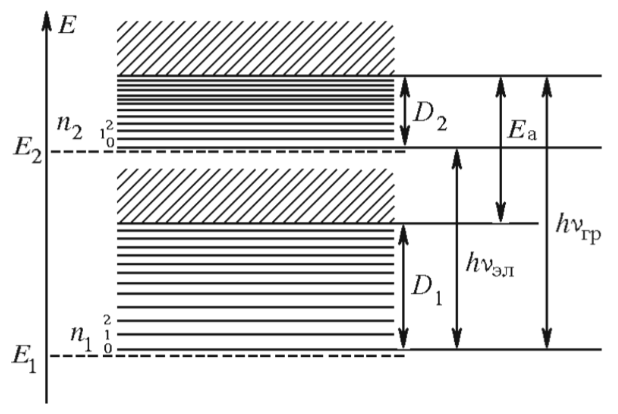
\includegraphics[width = 0.37\textwidth]{1.png}
	\centering
	\caption{Линии молекулы йода.}
	\end{wrapfigure}

	где $R = 109677.6~\text{см}^{-1}$ -- константа, называемая постоянной Ридберга, а $m$ и $n$ -- целые числа. Мы будем изучать серию Бальмера, линии которой лежат в видимой области. Для неё $n = 2$, а $m = 3,~4,~5,~6\dots$ Первые четыре линии обозначаются соответственно $H_\alpha$, $H_\beta$, $H_\gamma$, $H_\delta$.
	Для молекулы йода мы рассматриваем только нулевую серию, энергетическое положение линий поглощения определяется выражением
	\begin{equation}
	h\nu_{0, n_2} = (E_2 - E_1) + h\nu_2 \left( n_2 + \dfrac{1}{2} \right) - \dfrac{1}{2} h \nu_1.
	\end{equation}
	\subsection*{Описание установки}
	Для наблюдения спектра водорода используется установка, изображённая на Рис. 2А. Источником света для наблюдения служит водородная трубка Н-образной формы, в состав газа которой добавлены водные пары для увеличения яркости интересующих нас линий. Источник Л помещается на оптическую скамью вместе с конденсером К, так что свет концентрируется на входной щели 1. Далее через коллиматорный объектив 2 свет попадает на сложную спектральную призму, состояющую из призм П$_1$, П$_2$ и П$_3$. Первые две призмы обладают большой дисперсией, а промежуточная П$_3$ поворачивает лучи -- такое устройство позволяет складывать дисперии П$_1$ и П$_2$. После прохождения призмы свет попадает в зрительную трубу 4-5, объектив которой даёт изображение входной щели различных цветов.
	\newpage

	\begin{figure}[h]
	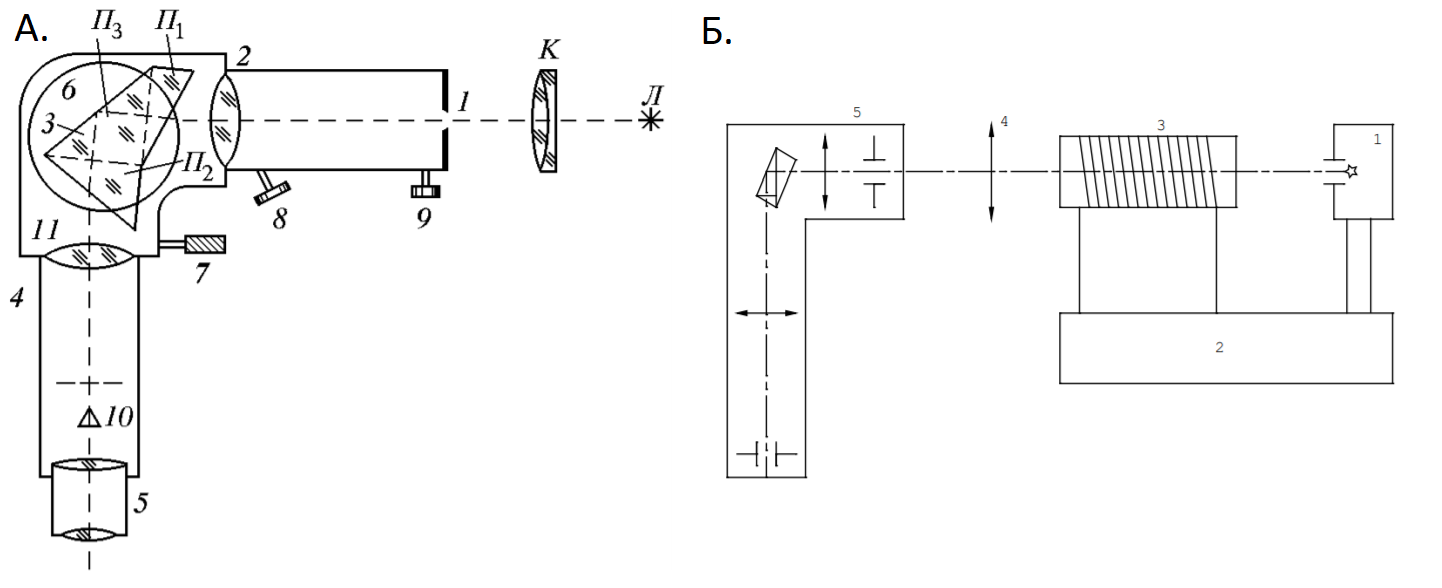
\includegraphics[scale=0.5]{2.png}
	\centering
	\caption{Установки для наблюдения линий А. водорода; Б. йода.}
	\end{figure} 

	На Рис. 2Б изображена схема установки, используемой для наблюдения спектра йода. Спектр поглощения паров йода наблюдается визуально на фоне сплошного спектра лампы накаливания 1, питаемой от блока питания 2. Кювета 3 с кристаллами йода подогревается нихромовой спиралью, подключённой вместе с лампой накаливания к блоку питания. Линза 4 используется как конденсор. В результате подогрева кристаллы йода частично возгоняются, образуя пары
	с лёгкой фиолетовой окраской. Спектрометр 5 позволяет визуально наблюдать линии поглощения молекул йода на фоне сплошного спектра излучения лампы накаливания видимой области.

	\section{Ход работы}
	\subsection*{Калибровка}
	Сначала произведём градуировку монохроматора. Для этого проведём измерения линий спектра неона и ртути, сняв зависимость длины волны наблюдаемого света $\lambda$ от параметра $\theta$ барабана монохроматора. Погрешность измерения $\theta$ примем половиной цены деления $\sigma_\theta = 5^\circ$. Измерения представлены в Таблице 1.
	\begin{table}[h]
		\centering
		\caption{Измерения для градуировки. Неон и ртуть.}
		\begin{tabular}{|c|c|c|c|c|c|} \hline
			$\lambda$, \AA	   & 5401 & 5852 & 5945 & 6143 & 6402 \\ \hline
			$\theta$, $^\circ$ & 1958 & 2216 & 2268 & 2360 & 2460 \\ \hline
		\end{tabular}
		
		\begin{tabular}{|c|c|c|c|c|c|c|c|c|} \hline
			$\lambda$, \AA      & 4047 & 4358 & 4916 & 5461 & 5770 & 5791 & 6234 & 6907 \\ \hline
			$\theta$, $^\circ$  &  380 &  922 & 1582 & 2000 & 2184 & 2196 & 2400 & 2650 \\ \hline
		\end{tabular}
	\end{table}

	Искать зависимость $\lambda = \lambda(\theta)$ будем в виде (дисперсионная формула Гартмана):
	$\lambda = \lambda_0 + \dfrac{C}{\theta - \theta_0}$
	График аппроксимации представлен на Рис. 3, полученные константы:

	$$\lambda_0 = (2179 \pm 15)\; \text{\AA} \qquad C = -(696 \pm 6) \cdot 10^4\; \text{\AA} \qquad \theta_0 = (4118 \pm 11)\; ^\circ$$
	
	\newpage

	\begin{figure}
	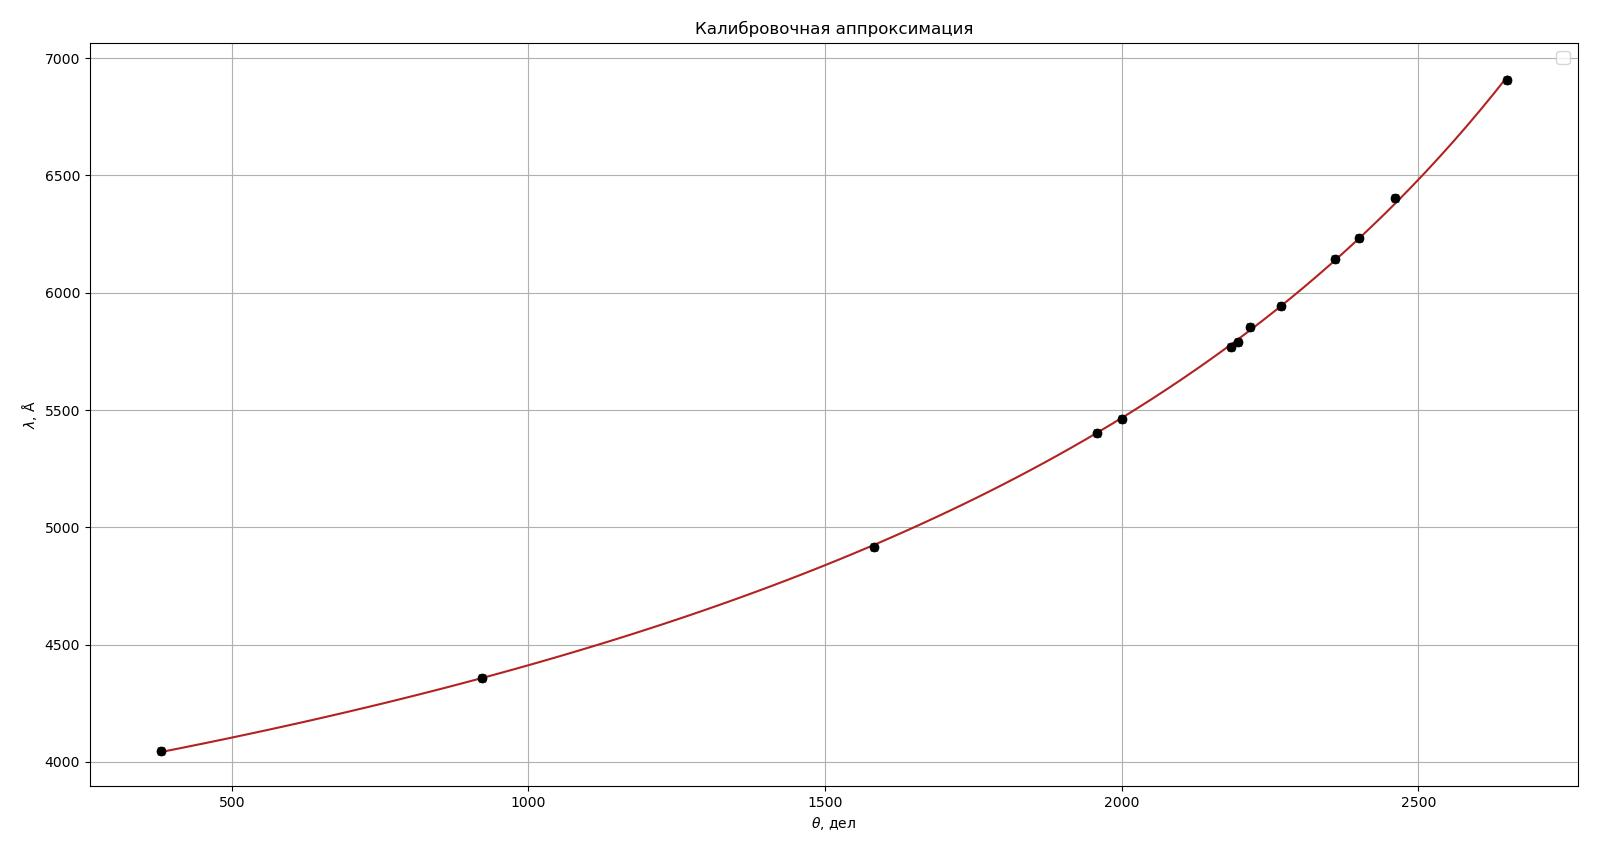
\includegraphics[width = 0.95\textwidth]{3.jpg}
	\centering
	\caption{Зависимость $\lambda = \lambda(\theta)$.}
	\end{figure}

	\subsection*{Водород}

	Произведём непосредственно измерения для серий водорода. Измеренные значения параметра барабана для $H_\alpha$, $H_\beta$, $H_\gamma$ и $H_\delta$:
	\begin{table}[h]
		\centering
		\caption{Водород}
		\begin{tabular}{|c|c|c|c|c|} \hline
			$\theta$, $^\circ$ & 568  &  898 & 1534 & 2534 \\ \hline
			$\lambda$, \AA	   & 4140 & 4341 & 4874 & 6574 \\ \hline
			$\lambda_{th}$, \AA& 4100 & 4340 & 4861 & 6563\\ \hline
		\end{tabular}
	\end{table}

	Воспользовавшись формулой (1), рассчитаем константу Ридберга для каждой из линий, итоговое значение:
	$$R = 110100 \pm 800~\text{см}^{-1}$$

	\subsection*{Йод}

	Перейдём к измерениям для йода. Параметры, соответствующие самой длинноволновой линии, линии, отстоящей от неё на 6, и границе спектра:

	\begin{table}[h]
		\centering
		\caption{Йод}
		\begin{tabular}{|c|c|c|c|} \hline
			$\theta$, $^\circ$ & 2326 & 2250 & 1818 \\ \hline
			$\lambda$, \AA	   & 6064 & 5906 & 5206 \\ \hline
		\end{tabular}
	\end{table}

	Энергии колебательного кванта возбуждённого состояния молекулы йода:
	\[h\nu_{2} = \dfrac{h\nu_{1,5} - h\nu_{1,0}}{5} = 0.012 ~\text{эВ}.\]
	Учитывая, что $h\nu_1 = 0.027~\text{эВ}$, с помощью формулы (2) рассчитаем энергию перехода
	\[h\nu_{\text{эл}} = h\nu_{(1,0)} - \dfrac{1}{2} h\nu_2 + \dfrac{3}{2} h\nu_1 = 2.13 ~\text{эВ}.\]
	Тогда энергии диссоциации частиц в основном и возбуждённом состоянии, с учётом того, что энергия возбуждения атома $E_A = 0.94~\text{эВ}$:
	\[D_1 = h\nu_{\text{гр}} - E_A = 1.47 \pm 0.02~\text{эВ},\]
	\[D_2 = h\nu_{\text{гр}} - h\nu_{\text{эл}} = 0.26 \pm 0.03~\text{эВ}.\]
	
	\end{document}